\documentclass[a4paper,12pt]{article}
\usepackage[utf8]{inputenc}
\usepackage[T1]{fontenc}
% \usepackage[brazil]{babel}
\usepackage{tikz}
\usetikzlibrary{mindmap,trees}
\usepackage{geometry}
\geometry{margin=1in}

\title{Mapa Mental: Redes Digitais e Sociedade}
\author{}
\date{}

\begin{document}

\maketitle

\begin{center}
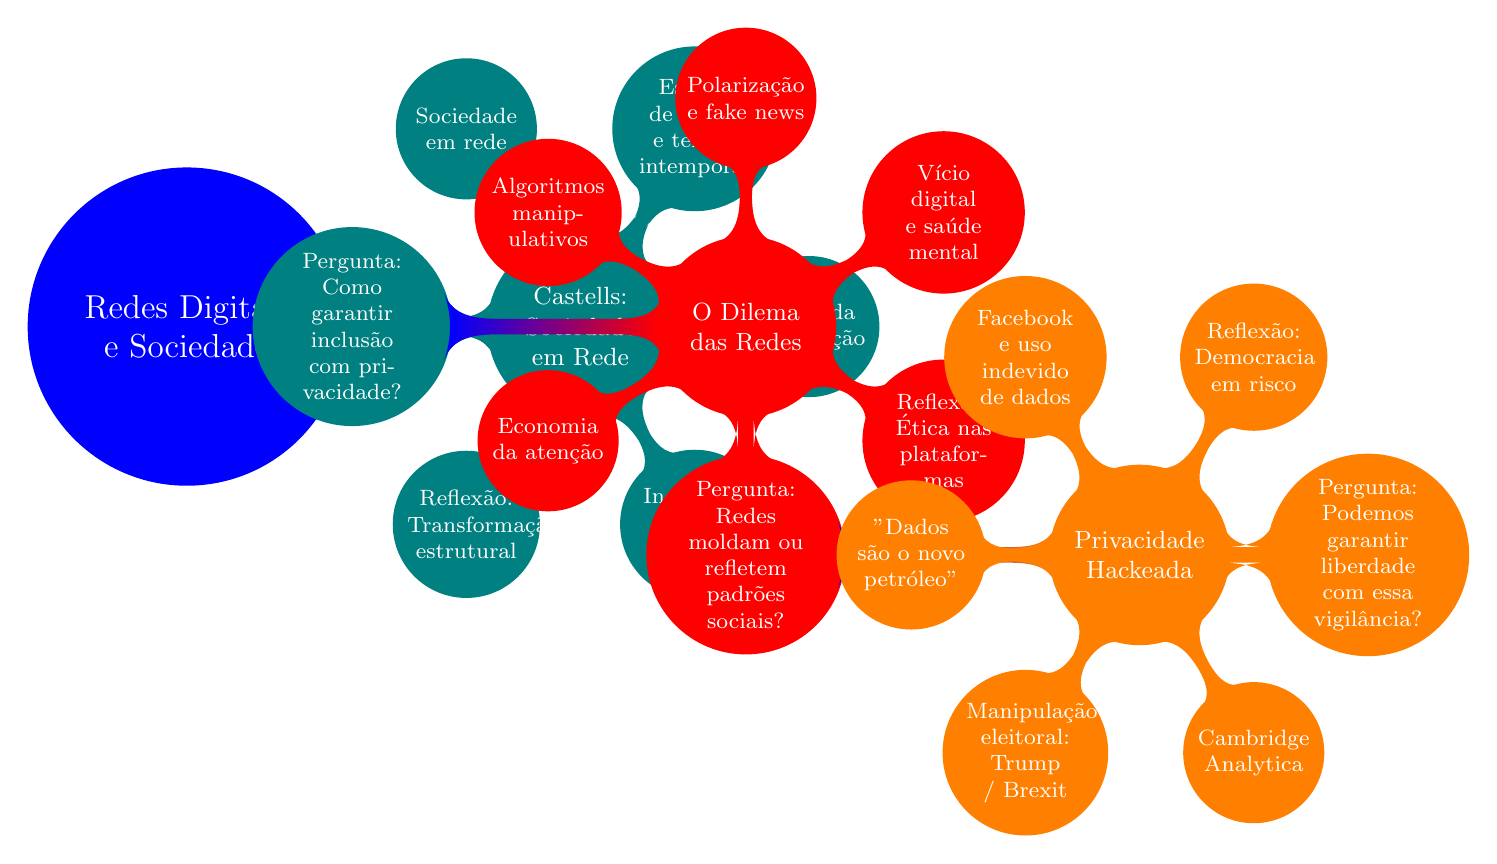
\begin{tikzpicture}
  \path[mindmap,concept color=blue,text=white]
    node[concept] {Redes Digitais e Sociedade}
    [clockwise from=0]

    % Livro: Castells
    child[concept color=teal] {
      node[concept] {Castells:\\ Sociedade em Rede}
      [clockwise from=120]
      child { node[concept] {Sociedade em rede} }
      child { node[concept] {Espaço de fluxos\\ e tempo intemporal} }
      child { node[concept] {Poder da informação} }
      child { node[concept] {Inclusão e exclusão digital} }
      child { node[concept] {Reflexão:\\ Transformação estrutural} }
      child { node[concept] {Pergunta:\\ Como garantir inclusão\\ com privacidade?} }
    }

    % Dilema das Redes
    child[concept color=red] {
      node[concept] {O Dilema das Redes}
      [clockwise from=210]
      child { node[concept] {Economia da atenção} }
      child { node[concept] {Algoritmos manipulativos} }
      child { node[concept] {Polarização e fake news} }
      child { node[concept] {Vício digital e saúde mental} }
      child { node[concept] {Reflexão:\\ Ética nas plataformas} }
      child { node[concept] {Pergunta:\\ Redes moldam ou\\ refletem padrões sociais?} }
    }

    % Privacidade Hackeada
    child[concept color=orange] {
      node[concept] {Privacidade Hackeada}
      [clockwise from=300]
      child { node[concept] {Cambridge Analytica} }
      child { node[concept] {Manipulação eleitoral:\\ Trump / Brexit} }
      child { node[concept] {"Dados são o novo petróleo"} }
      child { node[concept] {Facebook e uso indevido de dados} }
      child { node[concept] {Reflexão:\\ Democracia em risco} }
      child { node[concept] {Pergunta:\\ Podemos garantir liberdade\\ com essa vigilância?} }
    };

\end{tikzpicture}
\end{center}

\vspace{1cm}

\section*{Conexões entre os Ramos}
\begin{itemize}
  \item \textbf{Castells + Dilema das Redes:} A lógica em rede permite controle da atenção e manipulação algorítmica.
  \item \textbf{Castells + Privacidade Hackeada:} O poder da informação se concretiza no uso político dos dados.
  \item \textbf{Dilema das Redes + Privacidade Hackeada:} Ambos denunciam o uso antiético dos dados e a falta de regulamentação.
\end{itemize}

\section*{Responsabilidades Éticas (ADS / TPG)}
\begin{itemize}
  \item Desenvolver sistemas com foco na dignidade humana.
  \item Garantir transparência e segurança no uso de dados.
  \item Recusar demandas que envolvam manipulação de comportamento.
  \item Pensar ética desde o início dos projetos.
\end{itemize}

\section*{Ações Pessoais e Profissionais}
\begin{itemize}
  \item \textbf{Como cidadão:} usar navegadores seguros, controlar permissões de aplicativos, entender políticas de privacidade.
  \item \textbf{Como profissional:} respeitar a LGPD, promover justiça algorítmica, proteger o usuário final.
\end{itemize}

\end{document}
